\documentclass[12pt,a4paper]{report}
\synctex=1
\usepackage[utf8]{inputenc}
\usepackage[margin=2cm, top=1.5cm, bottom=2cm]{geometry}
\usepackage{graphicx}
\usepackage{libertine}
\usepackage{amsmath}
\usepackage{amssymb}
\usepackage{listings}
\usepackage{pgfornament}
\usepackage{eso-pic}
\usepackage{textcomp}
\usepackage{courier}
\usepackage[hangul]{kotex}

\title{
	\centering
	\pgfornament[width=12cm,color=teal]{84}\\
	\vspace{1cm}
	\fontsize{50}{50} \selectfont {오목 인공지능 형성\\설계과제 수행 계획서}\\
		\pgfornament[width=12cm,color=teal]{88}\\
	\vfill}
\author{
	\LARGE
	\begin{tabular}{rl}
		\hline
		교과목명 : & 자료구조와 실습\\
		담당교수 : & 정 준호 교수님\\
		프로젝트명 : & $\Omega$目\\
		학번 : & 2016110056\\ 
		이름 : & 박승원\\
		날짜 : & \today\\
		\hline
		\vspace{1cm}
	\end{tabular}
\\	

\includegraphics[width=0.5\textwidth]{logo.jpg}
	}
\date{}


\linespread{1.3}

\begin{document}

\lstset{language=C, columns=flexible, tabsize=4, frame=shadowbox, showstringspaces=false, breaklines=true, upquote=true, basicstyle=\ttfamily}

\maketitle

%\includegrap

\newpage
\tableofcontents

\noindent
%\chapter{설계과제 개요}
%\section{과제 목표}
%\section{과제 내용}
%\subsection{개발 설계}
%\subsection{프로그램 구현}
%\subsection{마무리}
%\section{과제 수행 방법}
\chapter{설계과제 개요}

\section{과제 목표}
최소한의 룰을 입력한 후, 스스로 학습하여 실력을 늘려가는 오목 게임 인공지능.
\section{과제 내용}
최근에 알파고라는 센세이셔널한 열풍이 휩쓸고 지나갔다. 
컴퓨터가 스스로 대국을 두어가며, 실력을 늘려갈 수 있다는 아이디어는 매우 신선했다.
이에 그런 비슷한 프로그램을 한 번 만들어 보면 어떨까 하는 생각이 떠올랐다.

우선은 오목의 가장 기본 규칙인 다섯 개를 연달아 놓으면 이긴다는 가장 단순한 규칙을 주고, 그 이외에는 컴퓨터끼리 대국하여 실력을 늘려가는 방식을 차용하기로 했다.

물론, 알파고의 인공 지능처럼 방대한 연산 능력이나, 고차원적인 알고리즘은 할 수 없지만, 그냥 단순히 기보를 기억하고, 그 승패의 결과를 누적해도 오목은 단순한 게임이기에 어느 정도의 인공지능은 달성할 수 있으리라 생각된다.
\subsection{개발 설계}
\begin{itemize}
\item char board[20][20]의 바둑판 위에 문자로 OX로 바둑돌을 표시한다.
\item 바둑판을 분석하여 승패를 결정짓는 위치를 알아낼 수 있게 한다.
\item 그러한 결정적인 위치가 없을 경우에는 현재 놓인 바둑돌의 2칸 이내의 랜덤한 위치에 바둑돌을 놓고 그 기보를 기억한다.
\item 최종적으로 승패가 결정되었을 때에 그 판에 둔 모든 random한 바둑돌들의 데이터를 승패로 결정하여 누적한다.
\item 컴퓨터끼리 많은 대국을 하여 데이터를 누적한다.
\item 이렇게 누적한 데이터를 바탕으로 인간과 둘 때에, 각 위치의 승률을 따져서 높은 곳을 선택한다.
\end{itemize}
\subsection{프로그램 구현}
\begin{itemize}
\item 기보 데이터는 매우 많은 경우의 수가 있으므로, 데이터가 매우 크리라 생각된다.
그러므로, 기보 저장시 압축하는 알고리즘을 사용한다.
\item 압축한 기보 데이터를 해싱과 이진 트리를 사용하여, 저장하고, 검색할 수 있게 한다.
\item 텍스트로 보드를 표현한다.
\end{itemize}
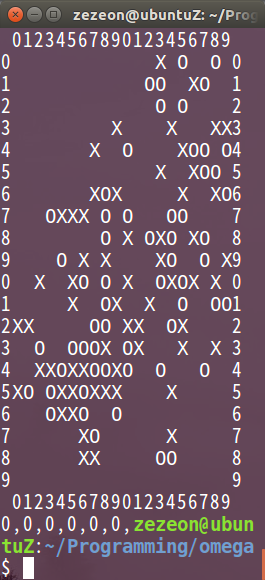
\includegraphics[width=0.4\textwidth]{b.png}
\subsection{마무리}
\begin{itemize}
	\item 어느 정도의 인공지능이 형성되었는지 평가한다.
\end{itemize}

\section{과제 수행 방법}
C언어로 프로그램을 작성하기로 했다.
혼자서 프로젝트를 진행하기로 하였으므로, 시간이 나는 틈틈이 프로그램을 짜기로 하였다.



\chapter{설계과제 목표 및 주요 내용}
\section{과제 목표}
학습형 오목 인공지능.
\section{과제 내용}
\subsection{개발 설계}
\subsubsection{계획서 작성}
현재까지는 바둑돌의 배열을 분석하여 결정적 위치를 찾는 것과, 임의의 위치에 바둑돌을 두는 것, 바둑판을 압축하여 표현하고 다시 원상 복구하는 것, 컴퓨터끼리 대국을 두는 것을 구현하였다.

기보를 승패의 결과에 따라 저장하고, 컴퓨터끼리 둔 대국의 데이터를 바탕으로 수를 결정하는 부분이 남았다.
이 부분은 해싱과 트리로 구현할 생각이므로, 시간이 좀 걸리리라 생각된다.
\subsubsection{요구사항 검토}
이 프로그램은 인공 지능 형성이 목적이므로, 텍스트로 평이하게 바둑판을 표현하고, 가로 세로 좌표를 콘솔로 입력하는 것으로 바둑돌을 두는 인터페이스를 선택하였다.
\subsubsection{모듈 설계}
\begin{itemize}
\item 현재의 바둑판을 압축하고 푸는 함수
\item 오목 룰에 따라 승패를 결정하는 결정적인 포인트를 찾아내는 함수
\item 랜덤한 위치에 바둑돌을 두는 함수
\item 기보를 해싱과 이진트리를 이용하여 저장하고 검색하는 함수
\item 컴퓨터끼리 대국을 두거나 인간을 상대로 두는 인공 지능 함수
\end{itemize}

\subsection{프로그램 구현}
\lstinputlisting[caption={기보를 압축하고 푸는 함수}]{src/compress.c}
\lstinputlisting[caption={find\_straight() 바둑판에서 원하는 바둑돌의 배열을 찾아내는 함수}]{src/find.c}
\lstinputlisting[caption={결정적 위치가 있을 경우 그 위치를 선택하고, 없을 경우에 랜덤한 위치를 선택하는 원초적 인공지능 함수, 이렇게 누적한 데이터를 바탕으로 나중에 좀 더 세련된 인공지능을 형성한다.}]{src/ai.c}
\subsection{마무리}
\begin{itemize}
\item 인공지능의 수준을 평가한다.
\item 개선할 만한 사항을 살펴본다.
\item 더 나은 알고리즘에 대해 생각해 본다.
\end{itemize}
\section{과제 수행 방법}
\begin{itemize}
\item C언어로 전적으로 작성하기로 하였다. 
\item 모듈화를 최대한 하여 버그를 줄이도록 노력한다.
\item 큐, 트리, 해싱 등의 자료구조를 최대한 활용한다.
\end{itemize}
\chapter{과제 수행 일정}
\begin{tabular}{|c|c|}
	\hline
세부 개발내용&주별 세부 추진 일정\\
\hline
자료수집 및 설계 계획 수립&$\sim$ 11/16\\
요구사항 검토&11.17\\
구조도 및 모듈 설계&11.18\\
프로그램 설계&11.19\\
프로그램 코딩&11.20$\sim$ 11.25\\
성능확인 및 오류 수정&11.26$\sim$ 11.30\\
최종 점검 및 개선 사항 보완&12.1\\
\hline
\end{tabular}
\end{document}
